\documentclass[tikz, border=2mm]{standalone}
\usepackage{tikz}
\usetikzlibrary{shapes, arrows.meta, positioning, backgrounds, calc}

\definecolor{rwthblue}{HTML}{00549f}
\definecolor{rwthmediumblue}{HTML}{3276b4}
\definecolor{rwthlightblue}{HTML}{6499c8}
\definecolor{rwthverylightblue}{HTML}{95bbdd}
\definecolor{rwthveryverylightblue}{HTML}{C7DDF2}
\definecolor{rwthveryveryverylightblue}{HTML}{ddeaf7}
\definecolor{rwthgreen}{HTML}{57AB27}
\definecolor{rwthmediumgreen}{HTML}{72b544}
\definecolor{rwthlightgreen}{HTML}{8DC060}
\definecolor{rwthverylightgreen}{HTML}{bad99f}



\begin{document}

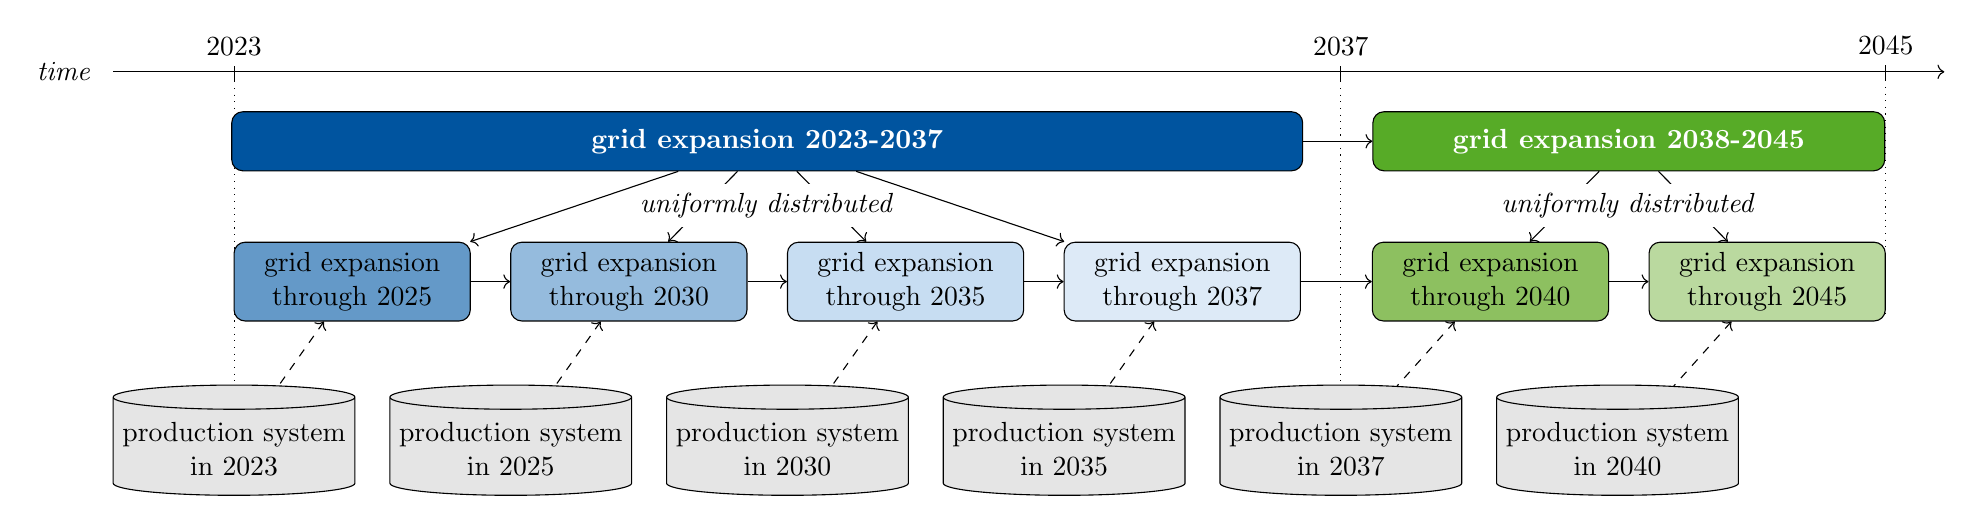
\begin{tikzpicture}[node distance=0.4cm and 0.5cm,
                    auto, 
                    expansionperiod/.style={rectangle, draw, align=center, rounded corners, minimum height=0.75cm, minimum width=3cm},
                    subexpansionperiod/.style={rectangle, draw, align=center, rounded corners, minimum height=1cm, minimum width=3cm},
                    database/.style={cylinder, shape border rotate=90, aspect=0.1, draw, align=center, minimum height=1.4cm, minimum width=3cm, fill=gray!20}]

    % Main Nodes
    \node[subexpansionperiod, fill=rwthlightblue, xshift=1.5cm] (2023) {grid expansion\\through 2025};
    \node[subexpansionperiod, fill=rwthverylightblue, right=of 2023] (2025) {grid expansion\\through 2030};
    \node[subexpansionperiod, fill=rwthveryverylightblue, right=of 2025] (2030) {grid expansion\\through 2035};
    \node[subexpansionperiod, fill=rwthveryveryverylightblue, right=of 2030] (2035) {grid expansion\\through 2037};
    \node[subexpansionperiod, fill=rwthlightgreen, right=of 2035, xshift=0.4cm] (2037) {grid expansion\\through 2040};
    \node[subexpansionperiod, fill=rwthverylightgreen, right=of 2037] (2040) {grid expansion\\through 2045};

    \node[expansionperiod, fill=rwthblue, text=white, above=of $(2023)!0.5!(2035)$, yshift=1cm, minimum width=13.6cm] (2023-2036) {\textbf{grid expansion 2023-2037}};
    \node[expansionperiod, fill=rwthgreen, text=white, above=of $(2037)!0.5!(2040)$, yshift=1cm, minimum width=6.5cm] (2037-2044) {\textbf{grid expansion 2038-2045}};

    % Databases Nodes
    \node[database, below=of 2023, yshift=-0.4cm, xshift=-1.5cm] (db2023) {production system\\in 2023};
    \node[database, below=of 2025, yshift=-0.4cm, xshift=-1.5cm] (db2025) {production system\\in 2025};
    \node[database, below=of 2030, yshift=-0.4cm, xshift=-1.5cm] (db2030) {production system\\in 2030};
    \node[database, below=of 2035, yshift=-0.4cm, xshift=-1.5cm] (db2035) {production system\\in 2035};
    \node[database, below=of 2037, yshift=-0.4cm, xshift=-1.9cm] (db2037) {production system\\in 2037};
    \node[database, below=of 2040, yshift=-0.4cm, xshift=-1.9cm] (db2040) {production system\\in 2040};

    % Connecting lines for databases
    \draw[<-, dashed] (2023) -- (db2023);
    \draw[<-, dashed] (2025) -- (db2025);
    \draw[<-, dashed] (2030) -- (db2030);
    \draw[<-, dashed] (2035) -- (db2035);
    \draw[<-, dashed] (2037) -- (db2037);
    \draw[<-, dashed] (2040) -- (db2040);

    % Connecting lines for main periods
    \draw[->] (2023-2036) -- (2037-2044);
    \draw[->] (2023) -- (2025);
    \draw[->] (2025) -- (2030);
    \draw[->] (2030) -- (2035);
    \draw[->] (2035) -- (2037);
    \draw[->] (2037) -- (2040);

    % Arrows from 2023-2036 to subperiods
    \draw[->] (2023-2036) -- (2025);
    \draw[->] (2023-2036) -- (2030);
    \node[align=center, below=of 2023-2036, yshift=0.25cm, fill=white] {\textit{uniformly distributed}};
    \draw[->] (2023-2036) -- (2023);
    \draw[->] (2023-2036) -- (2035);
    \draw[->] (2037-2044) -- (2037);
    \draw[->] (2037-2044) -- (2040);
    \node[align=center, below=of 2037-2044, yshift=0.25cm, fill=white] {\textit{uniformly distributed}};

    % timeline
    \draw[->] ($(2023-2036.north west)+(-1.5, 0.5)$) -- ($(2037-2044.north east)+(0.75,0.5)$) 
        node[left, xshift=-23.4cm] {\textit{time}}; 
    
    \draw[] ($(db2023.north) + (0, 3.85)$) coordinate (tick2023) -- ++(0, 0.2) node[above] {2023};
    \draw[] ($(db2037.north) + (0, 3.85)$) coordinate (tick2037) -- ++(0, 0.2) node[above] {2037};
    \draw[] ($(2040.north east) + (0, 2.05)$) coordinate (tick2045) -- ++(0, 0.2) node[above] {2045};
    
    \begin{scope}[on background layer]
        \draw[dotted] (tick2023) -- ++(0, -5);
        \draw[dotted] (tick2037) -- ++(0, -5);
        \draw[dotted] (tick2045) -- ++(0, -3);
    \end{scope}
    
\end{tikzpicture}

\end{document}
